\chapter{Estimating Diffuse Horizontal Irradiance (DHI) from sky image}
\label{sec:my_work_chapter}
In this chapter, a new approach that we developed for estimating DHI from sky images is explained. First, our experimental setup and data is presented, then we talk about clear-sky model used here, and why estimating DHI is very important in predicting GHI. Furthermore, DHI estimation using the irradiance sensors and also sky-images is discussed. Afterwards, machine learning regression methods for obtaining DHI from sky-image are studies. Finally, the general strategy for power prediction in a photovoltaic power plant using the forecast irradiance components is proposed.

\section{Experimental Setup}
This study is conducted on one of the photovoltaic(solar) power plants operated by ABB company. This PV plant which is located in Cavriglia region in Italy is chosen as a pilot site for the "forecasting power prediction using sky-imagery" project. Therefore, it is equipped with the following instruments for recording irradiation and sky images:
\begin{itemize}
\item A customized wide-angle high resolution (4MP) camera system with a fisheye lens covering 185 degrees of field of view. The camera is in a packaging attached to a pole on rooftop of the building next to the site. Figure \ref{fig:camera_on_site} shows the camera and its position next to the PV plates.
\item Two GHI pyranometer (irradiance sensor); located close to the camera on rooftop. One of the sensors is horizontally facing sky, and the other one facing north with around 40 degrees angle to the horizontal plane. It's worth mentioning that the PV plates are titled to south with a fixed angle around 30 degrees to get more sun exposure.  Th sensors are depicted in Figure \ref{fig:pyranometers}.
\item A thermometer for recording the temperature at the site.
\item A PC which is connected to the camera, pyranometers and thermometer via their software interfaces in order to configure sample rates and store taken images and irradiance measurements. The data of power generated by the PV plant is also sampled and stored for every day. All the data recorded during each day is been automatically transfered to the company samba sever at midnight using a control software running on the PC.
\end{itemize}

\begin{figure}[h]
\caption{wide-angle camera system used at Carviglia site}
\label{fig:camera_on_site}
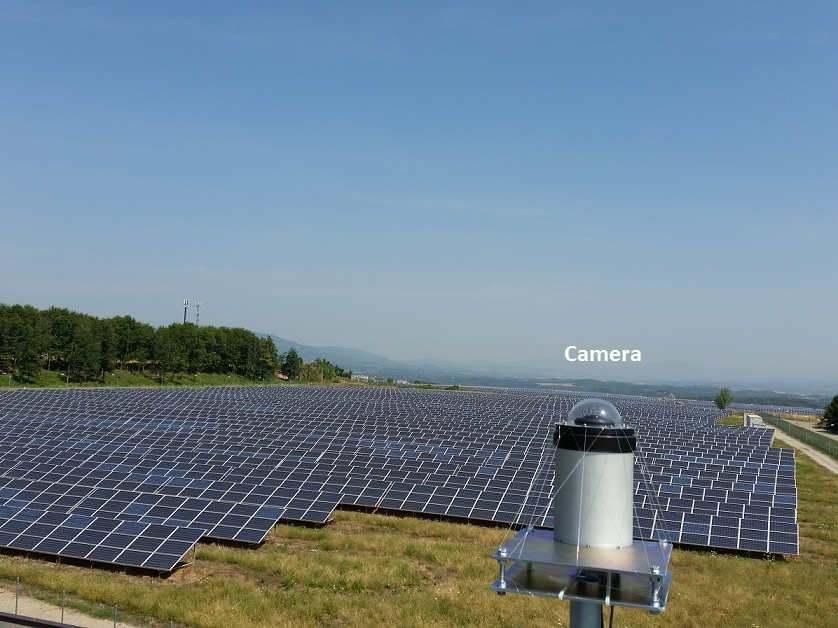
\includegraphics[scale=.3]{camera_on_site}
\centering
\end{figure} 

\begin{figure}[h]
\caption{Two pyranometers (one horizontal, one 45 degrees titled to north) located close to the camera location}
\label{fig:pyranometers}
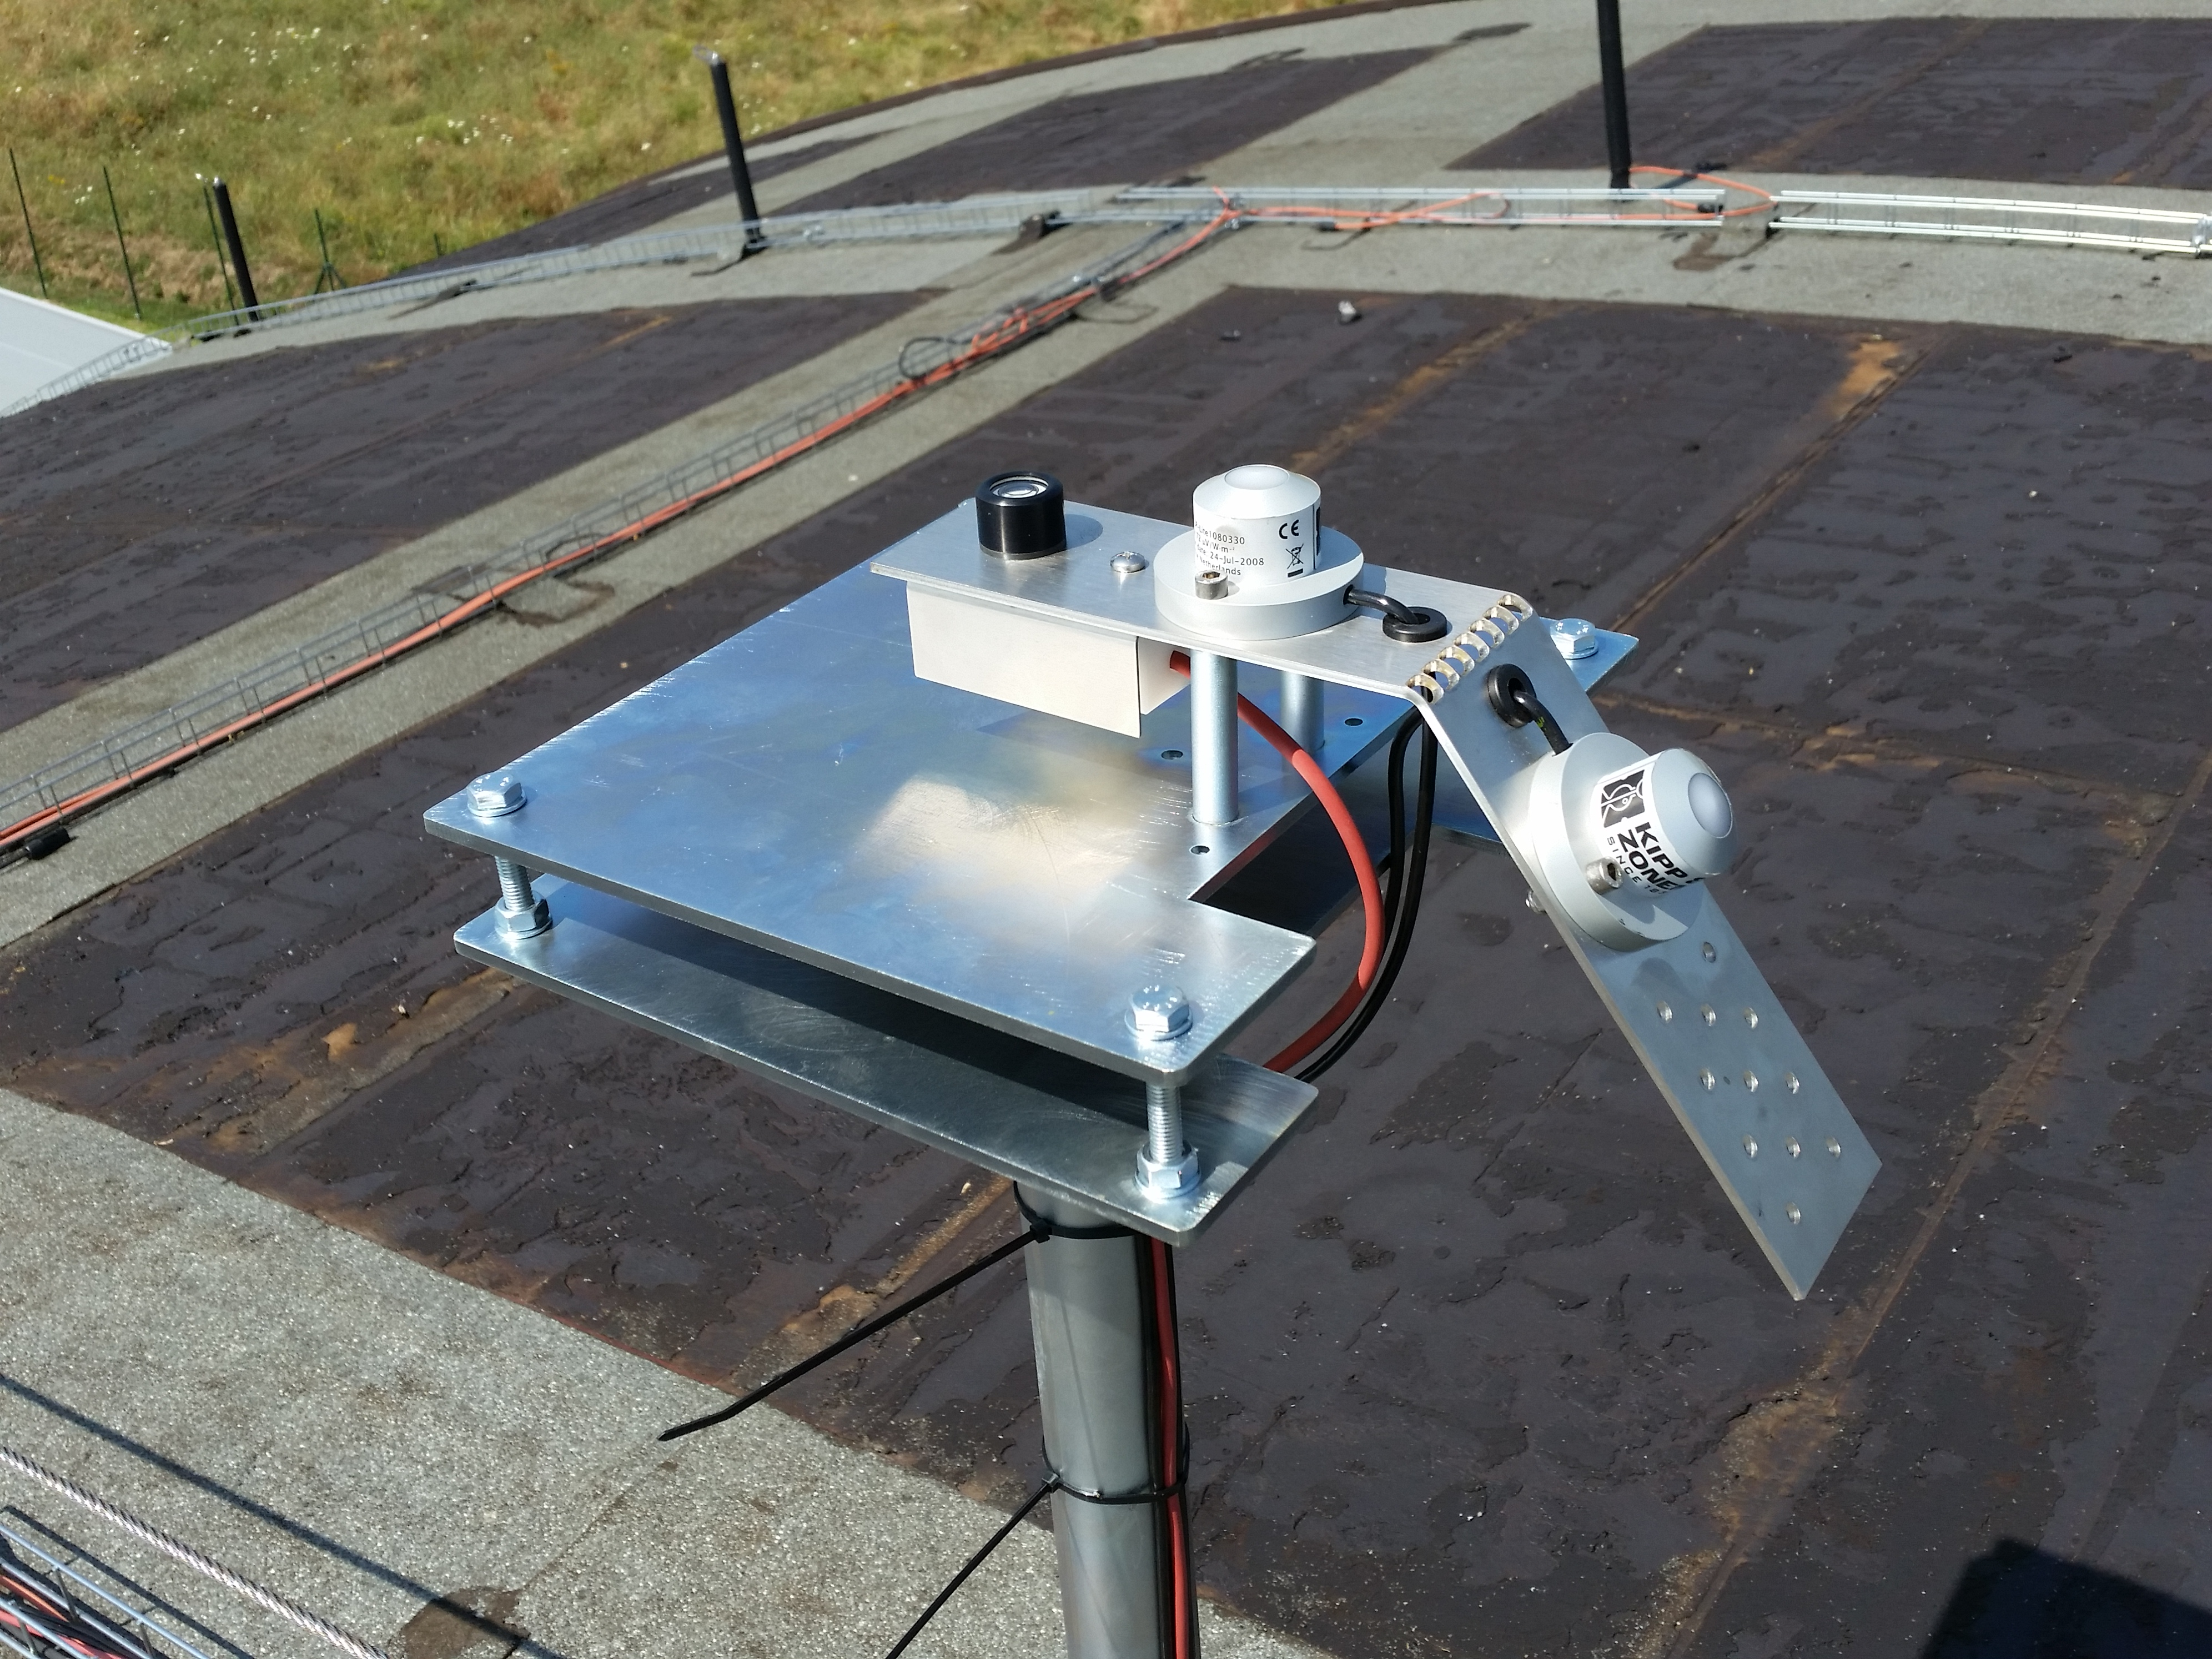
\includegraphics[scale=.3]{pyranometers}
\centering
\end{figure} 

\section{Acquired Data}
\label{sec:data}
The camera system captures several images from the whole-sky every 8 seconds with different narrow exposure ranges. These images which are labeled according to capture time, are combined to create an HDR (High Dynamic Range) image for every sample time. The original narrow exposure images are generally deleted except the images at each hour time (i.e. around 7:00, 8:00, 9:00 etc.). Since capturing images at night is not useful for power prediction applications, camera is instructed to only take pictures during daytime (i.e. sunrise to sunset) which is obtained for that specific location for each day using mathematical models. Nevertheless, according to the captures images, this is not enough and still there are some black images taken at the minutes before sunrise and after sunset. Therefore, while processing the images on the application side, we exclude those images using a threshold on average pixel intensity of each image. This threshold is determined empirically. The images are further filtered against a sky mask which is been designed to exclude nearby mountains and buildings in the field of view and also limit the field of view to 170 degrees since transforming the points which are further in horizon is not accurate enough and the sun light is not negligible when the sun is in those points.  It is worth mentioning that using HDR images in the image processing step is one of the key advantages of this study to related works specifically \cite{tSchmidt15}.

The pyranometers measure GHI values with the sample rate of 6 seconds. The temperature is also recorded with the  same sample rate. However, the generate power is measured and logged every 3 seconds. These different sample rate make it necessary to interpolate the available data to find the estimated data for a time which there is no data available. Therefore, we can assign total irradiance, temperature and generated power to any given image using its capture time. This data acquisition setup has been running since 7th July 2015 until present. However, there are some short periods of time (usually lasting several days up to two weeks) which one of the sensors (pyranometers or the camera) had problems or the power plant was not working to produce power data. Considering the relatively small sample rate (less than 8 seconds), the amount of recorded data is big enough to make those off-days negligible in data processing steps. The data used in this study spans from 15th July to 10 February, meaning that many summer, autumn and winter days are available in the dataset to make it a good representation for the whole year. 


\section{Sun positions and sun states in image}
\label{sec:sun-states}
Knowing position of sun is very important both in cloud segmentation and in irradiance estimation. First of all, since our images are from a wide-angle fisheye lens, they need to be transformed into geometric coordinates by an un-distortion algorithm to make them ready for further image processing steps including sun position, cloud segmentation and etc. This can be done by multiplying the raw image coordinates to camera transformation matrix which consists of intrinsic and extrinsic parameters of the camera system. As described in section \ref{sec:image_undistortion_schmidt}, intrinsic parameters are calculated using image of a chessboard\cite{fisheye_undistort} and extrinsic parameters are estimated using Kabsch algorithm\cite{Kabsch_alg} based on position of the sun appeared in the image versus the expected position of sun in image. The theoretical sun positions are calculated for the location of our PV plant site at every image time-stamp using NREL algorithm \cite{our_sun_position} in Matlab represented in unit sphere polar coordinates. As shown in Figure \ref{fig:sun_position_angles} this position is described as two angles (zenith and azimuth) which are converted to Cartesian coordinates using sphere to Cartesian conversion and later on are scaled to the image size to correspond with an image pixel. That pixel will be assumed as center of the sun.

\begin{figure}[h]
\caption{Sun position angles.  source:\cite{sun_angle_pic}}
\label{fig:sun_position_angles}
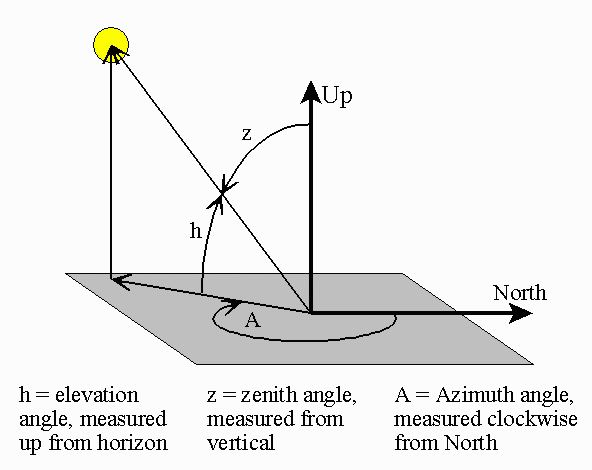
\includegraphics[scale=.5]{sun_angles}
\centering
\end{figure}

In cloud segmentation, which is not the focus of this study, sun position is used to treat pixels close to sun according to different threshold than other pixels. Furthermore, a sun state detection inspect the area around sun position to classify sun state in the image into following 4 categories:
\begin{itemize}
\item sun\_flag=4: indicating the sun is visible in the image and it appears as a star shape emitting 6 symmetric strong rays.
\item sun\_flag=3: indicating the sun is visible in the image and it appears as a star shape but with 5 or less symmetric strong rays.
\item  sun\_flag=2: indicating the sun is visible in the image but it does not appear as a star shape. Instead, it appears as a small black dot with no strong rays.
\item sun\_flag=1: indicating the sun is not visible in the image and it is either covered by clouds or the sun position is out of field of view in the image.
\item  sun\_flag=-1: indicating there is an unexpected situation around sun position, for example star shape sun is detected far away from expected sun position which could be because of strange cloud formations.
\end{itemize}
One sample for each one of these categories is depicted in Figure \ref{fig:sun_states}. We are able distinguish between this states thanks to HDR images, otherwise this fine classification would not be possible.

\begin{figure}[h]
\caption{Different sun states, from left to right: sun flag=4, 3, 2, 1 respectively.}
\label{fig:sun_states}
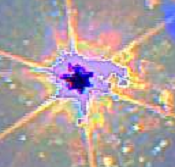
\includegraphics[scale=.5]{sun_flag_4}
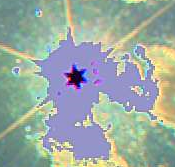
\includegraphics[scale=.5]{sun_flag_3}
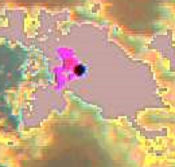
\includegraphics[scale=.5]{sun_flag_2}
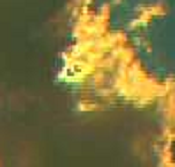
\includegraphics[scale=.5]{sun_flag_1}
\centering
\end{figure}

The variation of sun color in the images is so much that using Support Vector Machine for detecting sun is works very poorly. This issue is visible in Figure \ref{fig:sun_variation} which shows some clear sun samples from the images. Therefore, another approach using gray-scale images and geometrical symmetry detection is employed.

\begin{figure}[h]
\caption{Variation of sun appearance in the images.}
\label{fig:sun_variation}
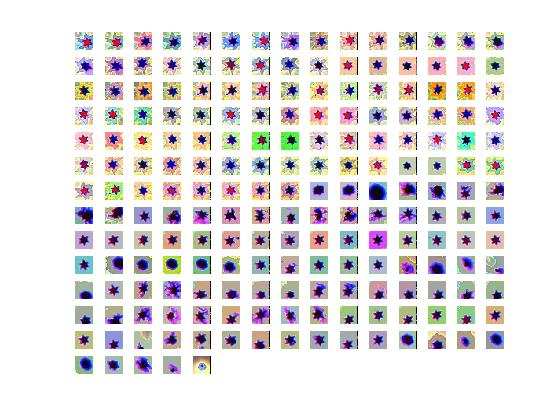
\includegraphics[scale=.7]{suns}
\centering
\end{figure}

Using these sun states along with the sun position in cloud segmentation algorithm, will lead to better segmentation results close to sun that is particularly a difficult area for cloud segmentation due to highly saturated pixels with different sky or cloud colors. In irradiance estimation which is the main focus of this study, sun position is used to create two specific feature vectors in a bounding circle around the sun. These features are explained section \ref{sec:img-features} in detail.

\section{Clear-sky irradiance model}
Before dealing with the problem of irradiance estimation from cloudy images we should know first know how much the irradiance would be at any time in clear sky conditions when there is no cloud in the sky at all. Fortunately, there are a few number of models which provide irradiance components at each given time for many locations on the Earth. In this study we investigate two of the these methods, Ineichen \cite{clear_sky_model} and McClear \cite{mcclear_alg}. Both of these methods use location coordinates (latitude, longitude) and query time (consisting of year,day,month,day,minute,second) to calculate sun angles internally and return the irradiation based on optic formulas which determine how much sun should reach the ground in as direct sunlight and how much should be scattered in hemisphere and forms the diffuse irradiance. The amount of scattered sunlight is varying throughout the year and also depends on the location, ground albedo\footnote{The fraction of solar energy (shortwave radiation) which is reflected from the Earth back into space. It is a measure of the reflectivity of the earth's surface. Ice, especially with snow on top of it, has a high albedo.} and aerosol parameters including pressure, ozone column content, water vapour column content,  optical depth and Angstrom coefficient. 

\subsection{Ineichen method}
Ineichen model statistically and physically relates some irradiance measurements to the aforementioned parameters as turbidity profiles which are available for different locations . We used the default turbidity values which come as a separate file in PV-Lib toolbox \cite{pv_lib_toolbox} in Matlab and is representative for most locations in Europe. However, one might need to use other appropriate turbidity profiles for other locations to get more accurate results.
 
\subsection{McClear method}
On contrary to this approach, McClear uses a fully physical model that exploits recent aerosol properties, total column content in water vapour and ozone produced by the MACC project (Monitoring Atmosphere Composition and Climate). The MACC project, funded by the European Commission, uses  data of many Numerical Weather Prediction (NWP) centers distributed around the world to provide a global aerosol property forecasts together with physically consistent total column content in water vapour and ozone. In other words, since McClear uses synthetic data of NWP's, it does not depend on any local atmospheric observations for irradiance prediction. For the sake of speed, McClear irradiance estimates are pre-computed for the the location of these measurement centers and are interpolated for all other point on th Earth using a look-up table approach. Of course the closer we are to one of these measurement centers, the more accurate McClear estimate will be. The McClear irradiance estimates are available worldwide for every minutes from 2004 to present with 2 days lag under this web service \cite{mcclear_site}. This means that if we want to get the irradiance for today, we need to interpolate data of several days or weeks before to get an estimate for the current time. Nevertheless, one can use the original data of past 2 days for current time as well, since irradiance does not change considerably in two days.

\subsection{Comparison of clear-sky simulation results}
\label{sec:compare-clear-sky-result}
To evaluate performance of these two clear-sky models we choose several days which have a significant clear part during the day (just because complete clear days are very rare). The chosen days should be from different months of year in order to represent performance of models for the whole year better. After observing the irradiance logs and images for verification, the following days were selected for comparison: 2015/07/19, 2015/08/03, 2015/09/21, 2015/10/24, 2015/11/24 and 2016/02/05. As an example, simulated GHI of three days are plotted in Figure \ref{fig:mcclear_vs_Ineichen_days} next to the observation. 

\begin{figure}[!ht]
\caption{GHI estimation of McClear vs Ineichen vs observation}
\label{fig:mcclear_vs_Ineichen_days}
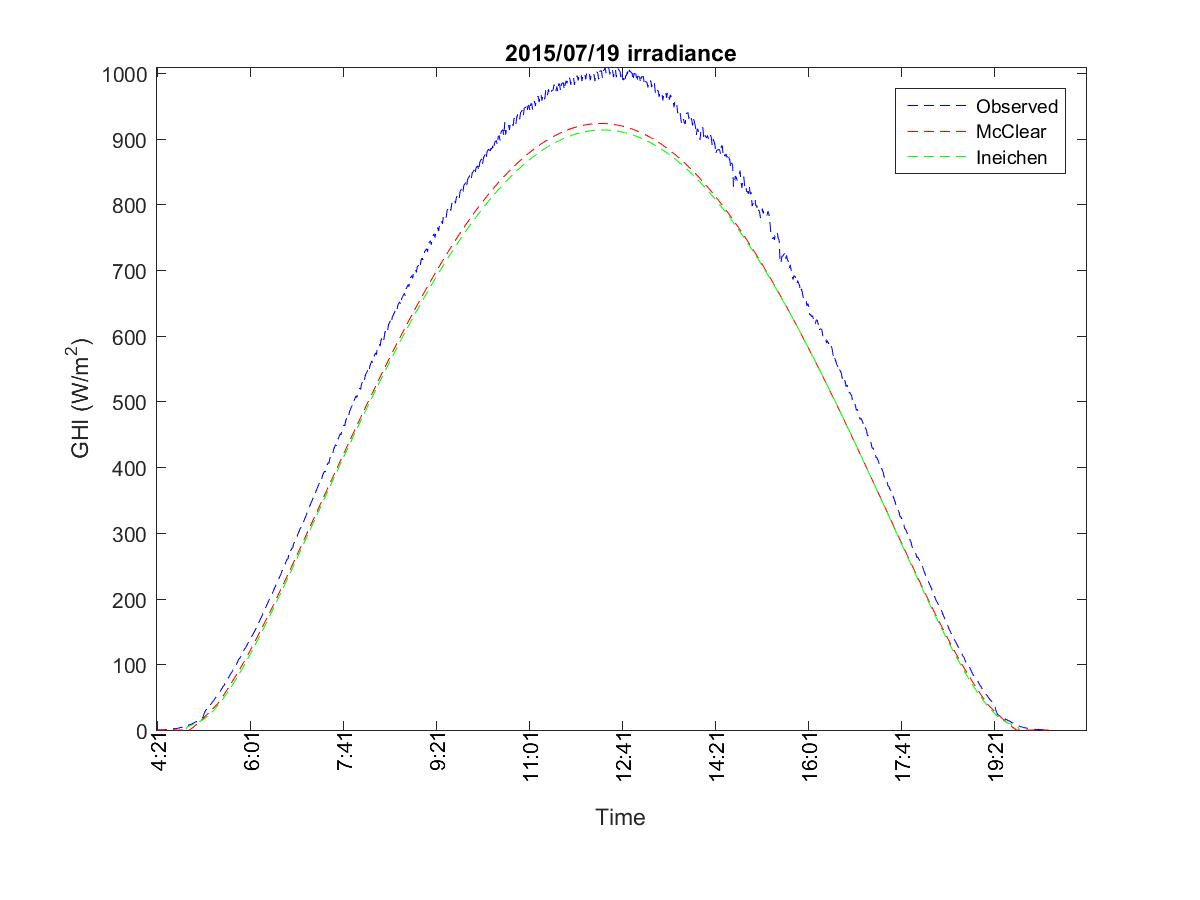
\includegraphics[scale=.2]{2015_07_19_irr}
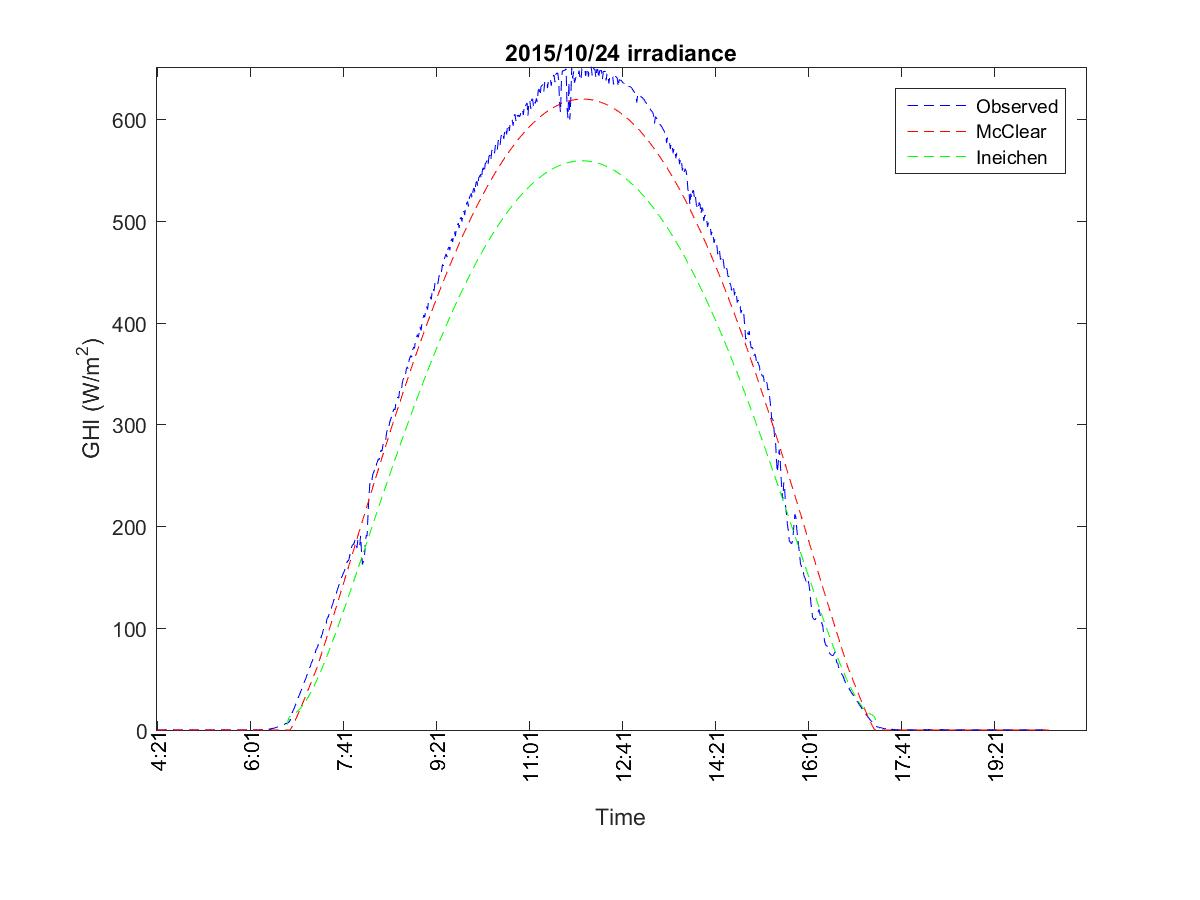
\includegraphics[scale=.2]{2015_10_24_irr}
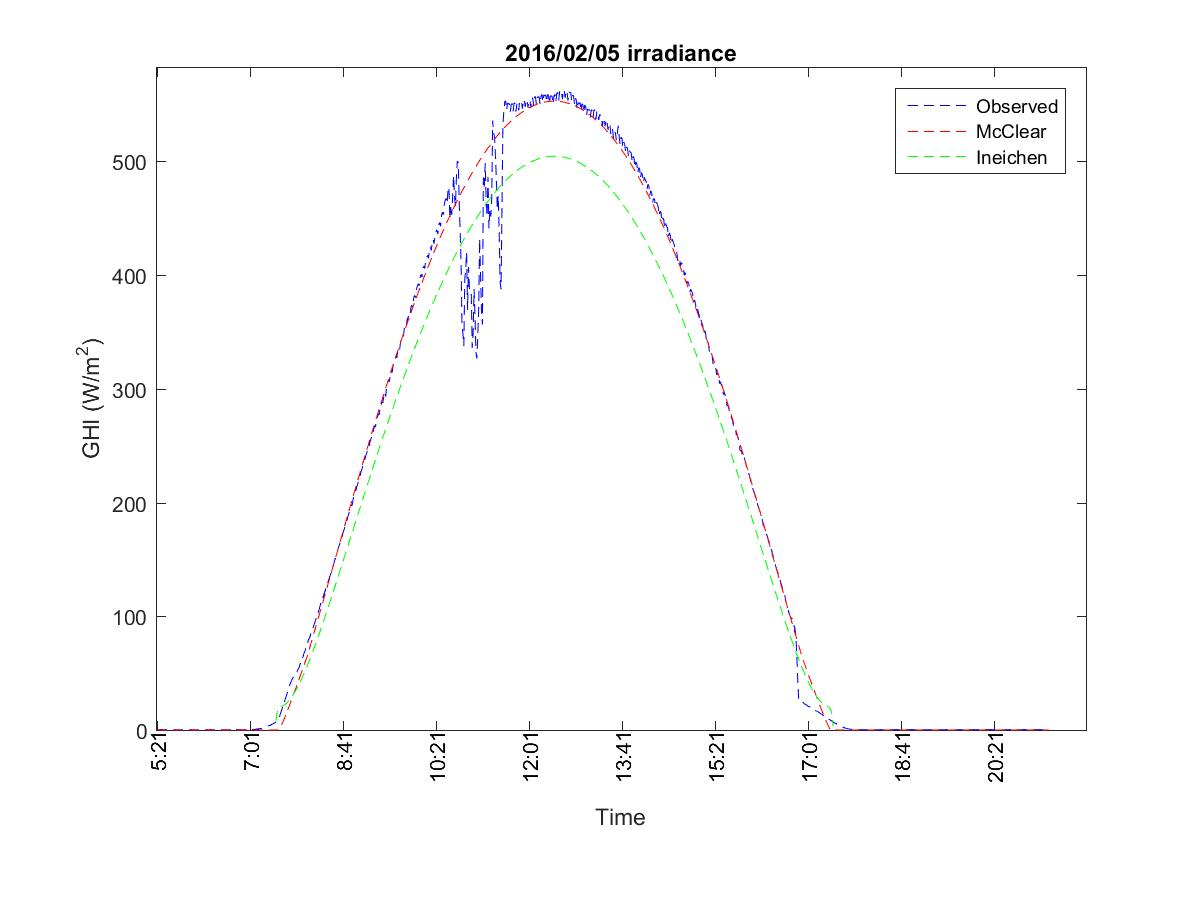
\includegraphics[scale=.2]{2016_02_05_irr}
\centering
\end{figure}

As it can be seen, both methods can predict the shape of irradiance curve very accurately around the year, but both have biases in the result such that the simulated values are always smaller than observed ones. During the summer days, McClear and  Ineichen results are biased almost equally, and as we get closer to winter days, the bias of McClear gets smaller and bias of Ineichen get slightly bigger. 
Figure \ref{fig:mcclear_to_Ineichen} shows the correlation of simulated GHI of both models plotted with respect to the actual measurements of all of the examined days.

\begin{figure}[h]
\caption{Correlation of GHI simulation of McClear and Ineichen with observations on selected days}
\label{fig:mcclear_to_Ineichen}
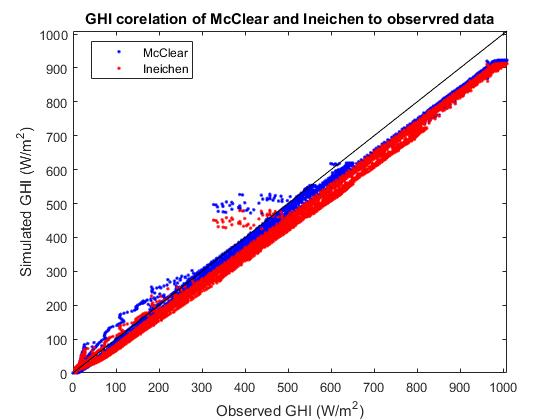
\includegraphics[scale=.7]{mcclear_inceichen}
\centering
\end{figure}

This plot again shows that the bias of McClear and Ineichen for large values of GHI is the same, and for small GHI values McClear result is closer to the observed irradiance. however, it also suggests that since Ineichen methods has lower variation in terms of bias, this bias can be compensated with a scaling factor more easily than the bias of McClear which shows larger variation throughout the year. Note that, the outliers in this figure are representing cloudy times. Furthermore, this bias of Ineichen method is strongly related to the turbidity factors that are neglected in our case by using the default values. It would be not surprising to see smaller bias if one uses turbidity factors which are verified for the location of PV plant. The correlation of DNI and DHI values of both methods are illustrated in Figure \ref{fig:mcclear_vs_Ineichen_DNI_DHI}. One can see that DNI is predicted much higher in Ineichen method and DHI is also simulated slightly higher than McClear values. This behavior is intensified during autumn for DNI, but it is not varying a lot for DHI. Since we do not have observation values of DHI and DNI, we cannot compare correlation of methods' results to the observed values in this figure.  However, we can hypothesize than during a complete sunny day, if at a very short time (i.e. seconds) a cloud covers the sun completely, the direct irradiance (DHI) is almost zero and all the irradiation only comes from DHI source which is the scattered light in the sky. Therefore, we can use our GHI irradiance observations as DHI and compare it to the DHI simulated values for that particular time. 


\begin{figure}[h]
\caption{DNI and DHI correlation of McClear to Ineichen}
\label{fig:mcclear_vs_Ineichen_DNI_DHI}
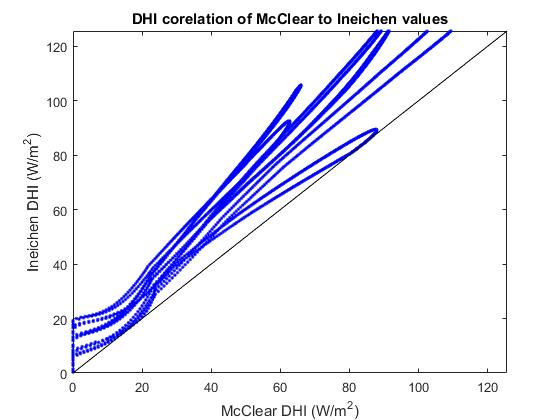
\includegraphics[scale=.4]{mcclear_inceichen_DHI}
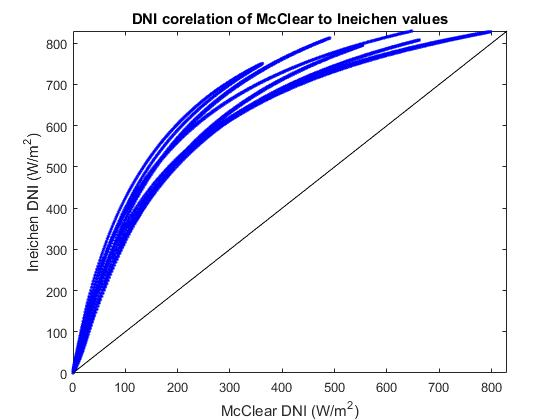
\includegraphics[scale=.4]{mcclear_inceichen_DNI}
\centering
\end{figure}

In Figure \ref{fig:McClear_DHI_vs_ineichen} this has been shown for a moment around 13:00 which sun is occluded by a small thick cloud and therefore, GHI is dropped rapidly to a value close to 150 which is very close to simulated DHI values from McClear and Ineichen methods. Also, there is no other cloud in the sky to influence the DHI component. Furthermore, the simulated DHI values are very close to each other at any time and resemble the shape of GHI relatively well during whole day. Thus, we can conclude that these models can predict DHI with good accuracy, and since DNI is a function of GHI and DHI according to Eq \ref{eq:irr_components}, DNI values calculated from McClear and Ineichen models are also accurate enough and for our application. This hypothesize has been verified by looking at many other data points where GHI observation gets very close to DHI simulation values and there is a cloud obstructing the direct sun light.

\begin{figure}[h]
\caption{Comparison of DHI of McClear and Ineichen to observed GHI}
\label{fig:McClear_DHI_vs_ineichen}
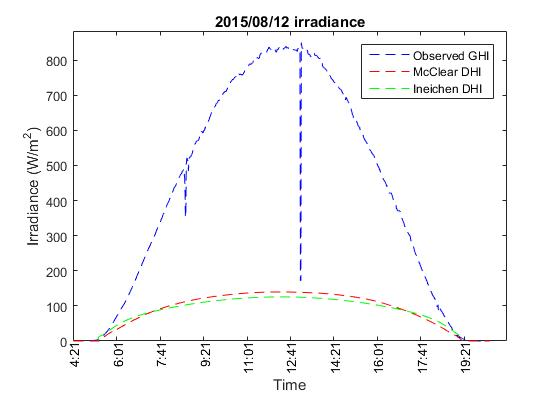
\includegraphics[scale=.5]{McClear_DHI_vs_ineichen}
\centering
\end{figure}

We know that DNI should be always larger than DHI during clear-sky condition. Looking at Figure \ref{fig:clean_sky_day_irr}, pattern of changes in the simulated values of DNI and DHI during a day confirms this condition too.

\begin{figure}[h]
\caption{Variation of irradiance components during day}
\label{fig:clean_sky_day_irr}
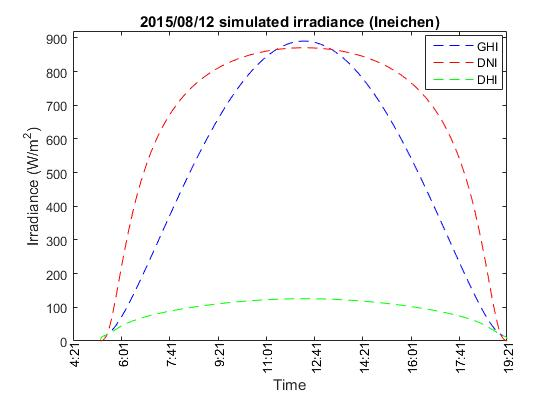
\includegraphics[scale=.5]{clean_sky_day}
\centering
\end{figure}

\subsection{Choosing the clear-sky model}
As we discuss in this chapter, McClear and Ineichen models both predict the clear-sky irradiance components relatively accurately,however the bias for Ineichen method is more robust and manageable than McClear bias. Furthermore, obtaining the McClear values requires downloading the irradiance files from their web service since there is not offline library for calculating them. All this considered together, we decided to use Ineichen as the clear-sky irradiance model for this study. The scaling factor for compensating the bias in Ineichen is set to 1.08 which is empirically calculated based on several clear day observations.

\section{Estimating diffuse from pyranometers}
After picking the suitable clear-sky model, we can predict the irradiance components for any given day in clear-sky conditions, but for determining the irradiation in cloudy conditions we need to first detect them and then find a relation between cloud states in the sky and the observed irradiance. Since GHI is composed of DHI and DNI, and because we want to get some hints from the images for determining GHI, the reasonable approach is to first estimate DNI and DHI values and then construct the GHI from them using sun zenith angle and Eq \ref{eq:irr_components}. Thus, for the learning algorithm we need DNI and DHI observations to relate them to image features. Ideally, we would have DHI and DNI observations separately along the GHI values from an advanced irradiance sensor\footnote{This type of pyranometers such as Zonen CM11 have a dynamic shade-band along the sun path to make sure that the sensor is always in shadow, this recording only DHI component. Then DNI can be computed from GHI and DHI or by using another type of pyranometer such as Eppley NIP.}, but in our experimental setup only GHI values are observed in horizontal and 40 degrees north. The idea behind putting one of the pyranometers tilted towards north is that based on sun path from an observant in that regions of the world, tilted surfaces toward the north do not get direct sun light during most of the day. That's why the PV plates are tilted towards the south to get more sunlight. The sun path at Cavriglia can be seen in Figure \ref{fig:cavriglia_sun_path}. There is a simple geometric rule that confirms this idea. If the angle between sun and the normal vector of a surface is greater than or equal to 90 degrees, sun rays which are coming straight from sun will not hit the surface. This condition will hold for many times during a day for the sensor with around 40 degrees tilt toward north.

\begin{figure}[h]
\caption{The sun path during a spring day at Cavriglia, Italy, location of ABB PV plant.}
\label{fig:cavriglia_sun_path}
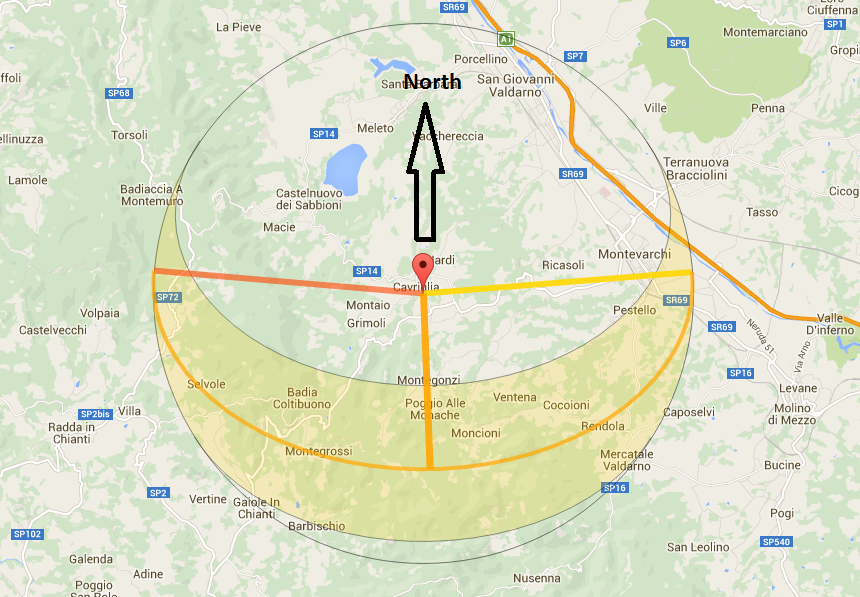
\includegraphics[scale=.5]{cavriglia_sun_path}
\centering
\end{figure}

Anyways, the sun path changes during the year, for example during the summer two edges of this path come higher towards north, and in winter they go lower towards south. This brings some direct sunlight to the tilted pyranometer in early morning and late evening during summer time. However, during winter and most of the autumn and spring, the tilted sensor is in complete shadow and does not receive direct sun irradiance (DNI). As a result, we can safely assume that during those times, the values recorded by this tilted sensor represent the diffuse irradiance component. This can be seen more clearly in Figure \ref{fig:tilted_irr_cmp}. In this picture, the dark blue curve represents irradiance observations of tilted sensor (sensor 1) during a sunny summer day -3th August. As one can see, around the morning and evening when the sun has a shine on the sensor, there is a bump in the irradiance. However, during rest of the day that the sensor goes into shadow, the irradiance is close to clear sky DHI. As we expect, during the winter the tilted sensor will be always shadowed, thus should not have any DNI part in its measurement during the whole day. Looking at Figure \ref{fig:tilted_irr_cmp2} confirms this idea, since there is no bump in the morning and evening records.

\begin{figure}[h]
\caption{Irradiance comparison of horizontal sensor (1) and tilted sensor (2) for a summer day}
\label{fig:tilted_irr_cmp}
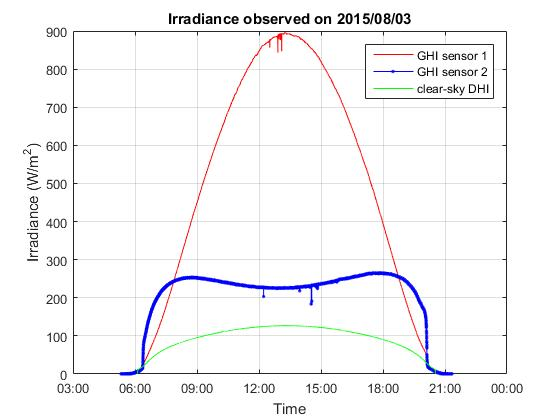
\includegraphics[scale=.4]{tilted_irr}
\centering
\end{figure}

\begin{figure}[h]
\caption{Irradiance comparison of horizontal sensor (1) and tilted sensor (2) for a winter day}
\label{fig:tilted_irr_cmp2}
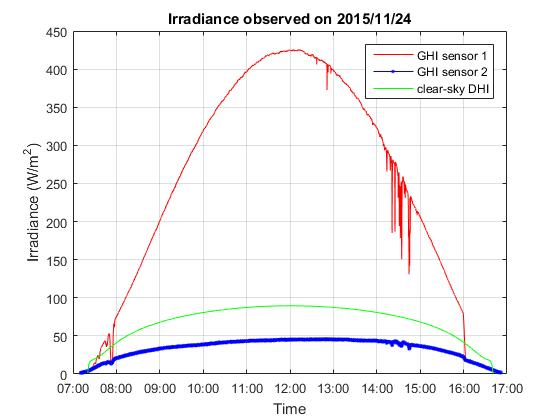
\includegraphics[scale=.4]{tilted_irr2}
\centering
\end{figure}

Therefore, if we deduct the direct irradiance component from sensor observations, we can obtain diffuse component which is required for our learning algorithm.  We previously have shown in \ref{sec:compare-clear-sky-result} that our DHI and DNI values obtained from clear-sky model have enough accuracy for this application. But for calculating the effective direct irradiance on tilted sensor we need to find the angle between sun and surface of the sensor at any time, since this angle is different than sun zenith. According to Figure we can use sun azimuth and sun zenith angles to locate the sun vector. The normal vector of tilted sensor surface can also be defined based on its zenith and azimuth angles. Then using this linear algebra equation \ref{eq:angle_sun_tilted} we can find the angle between two vectors in 3D space.

\begin{equation}
\label{eq:angle_sun_tilted}
\theta = Arctan2(\| a \otimes b \|, a \cdot b)
\end{equation} 
where Arctan2 is four quadrant arctangent of the elements.

However, for the horizontal sensor the effective direct irradiance can be simply computed as $DNI \times cos(zenith)$. We have shown in Figure \ref{fig:mcclear_vs_Ineichen_DNI_DHI} that DNI is almost zero(0) when the cloud occlude the sun completely. This case correspond to $sun\_flag=1$ as we explained in \ref{sec:sun-states}. And if the sun is completely shining like a star, hence resulting in full DNI, it corresponds to  $sun\_flag=4$. For other sun states where the sun is partially obstructed, the DNI is not the same as clear sky DNI. We hypothesize that the DNI for sun-flag=2 and 3 is somewhere between 0 and clear-sky DNI. However, for the sake of simplicity we do not consider these states in this study. In other words, we only try to estimate the DHI for the conditions that either sun is completely occluded ($DNI=0$) or it is completely visible and shining(i.e. $DNI=DNI_{clear\_sky}$. With this simplification we can compute the DHI for each irradiance sensor by re-writing Eq \ref{eq:irr_components} as:

\begin{equation}
\label{eq:DHI_eq}
DHI =
    \begin{cases}
      GHI - DNI \times cos (angle), & \text{if}\ sun\_flag=4 \\
      GHI, & \text{if}\ sun\_flag=1 \\
    \end{cases}
\end{equation}

where GHI is the observed total irradiance by the sensor, $angle=\theta$ for tilted sensor and $angle=zenith_{sun}$ for the horizontal sensor. Note that our experiment dataset is pruned to only contain image samples from these two sun-flags. Furthermore, we do not consider images for early morning (i.e before 8) and very late evening (i.e. after 19) for our training, since the GHI in those moments is very low -less than 100- which makes them insignificant for power generation and not interesting for our application. Plus that the pattern of sun in the horizon widely varies and result in unusual errors in our algorithms. Since the exact tilt angle of sensor 2 and its azimuth to the north is not given for sure, we need to evaluate a range of possible values to find the angles that bring results with less error during sunny days compared to $DHI_{clear\_sky}$.  The optimal angles found to be \textbf{57.5} degrees for zenith and \textbf{-0.7} degrees for azimuth. 
In Figure \ref{fig:calc_DHI_day}, calculated DHI values for a sunny summer and a sunny winter day are shown.

\begin{figure}[h]
\caption{Calculated DHI}
\label{fig:calc_DHI_day}
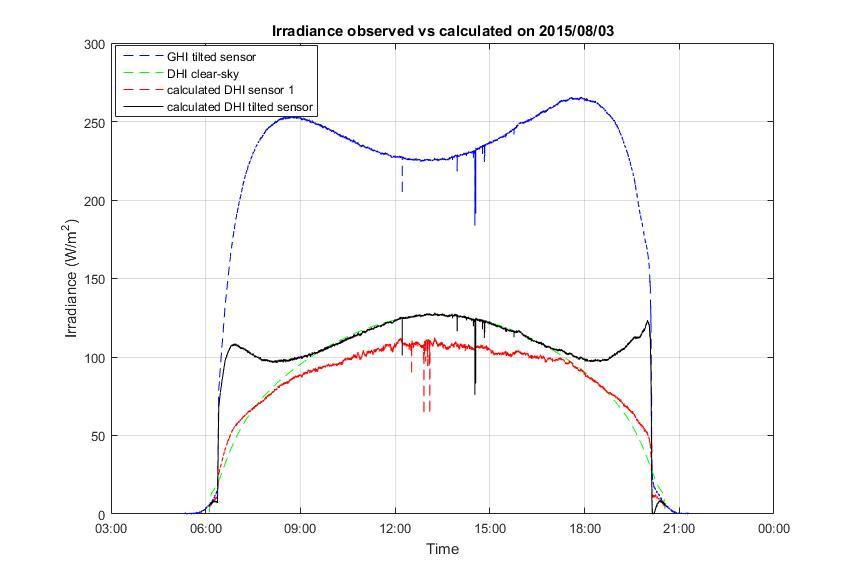
\includegraphics[scale=.4]{DHI_calced}
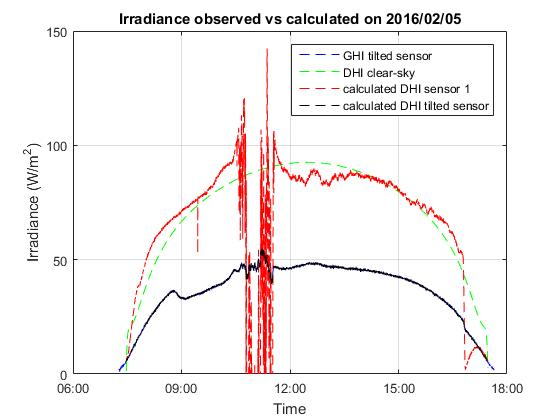
\includegraphics[scale=.8]{DHI_calced_winter}
\centering
\end{figure}

Interestingly, one can see two horn shape anomalies in the morning and evening on calculated DHI of a summer day. One hypothesize is that reflection of light from nearby mountains are causing this extra irradiance which is no accounted for in our model. Anyways, as we can see the DHI values of tilted sensor show more robustness compared to values of horizontal sensor. The reason is some complex effects of clouds on DNI which we are not considering so far. The tilted sensor is more immune to this DNI variation. Even though during the winter days, the calculated DHI for horizontal sensor is closer to clear-sky DHR, but the DHI of tilted sensor shows more robustness to cloud condition variations. Therefore, we decided to use DHI of titled sensor as actual DHI for both sensors on further calculations.

We also experimented reconstruction of observed irradiances for both sensors based on calculated DHI values (from tilted sensor), assumed DNI values and respective angles using Eq \ref{eq:GHI_reconstruct} . 

\begin{equation}
\label{eq:GHI_reconstruct}
\left[ \begin{array}{c} GHI_1 \\ GHI_2 \end{array} \right] = \begin{bmatrix} a_1 \times cos(zenith) & b_1 \\ a_2 \times max(0, cos(\theta)) & b_2 \end{bmatrix} \times \left[ \begin{array}{c} DNI \\ DHI \end{array} \right]
\end{equation}

where $GHI_1$ is irradiance reconstructed for horizontal senor (1), $GHI_2$ is the tilted sensor irradiance, $\theta$ is the angle between sun and tilted sensor normal, $a_1, a_2, b_1, b_2$ are constant values needed to be tuned for the best fit in result. For reconstruction we evaluated different values in range of 5 to 60 to find zenith and azimuth of the tilted sensor which result in best fit. Also, for the constant parameters the following values worked best: $a_1=0.9, a_2=1, b_1=1.14, b_2=0.78$. The optimal angles found to be \textbf{56.5} degrees for zenith and \textbf{11.5} degrees for azimuth which is different for the azimuth we used for obtaining the DHI values before (i.e. -0.7). However, we are only interested in reconstructing GHI for the horizontal sensor which does not depend on tilted sensor azimuth according to the aforementioned equation.

The correlation of reconstruction result to actual GHI values is shown in Figure \ref{fig:GHI_reconstruct_result} and proves that GHI values of horizontal (and tilted) sensor can be estimated using a simple DNI model and DHI of tilted sensor.


\begin{figure}[h]
\caption{Calculated GHI based on DHI and DNI for both sensors}
\label{fig:GHI_reconstruct_result}
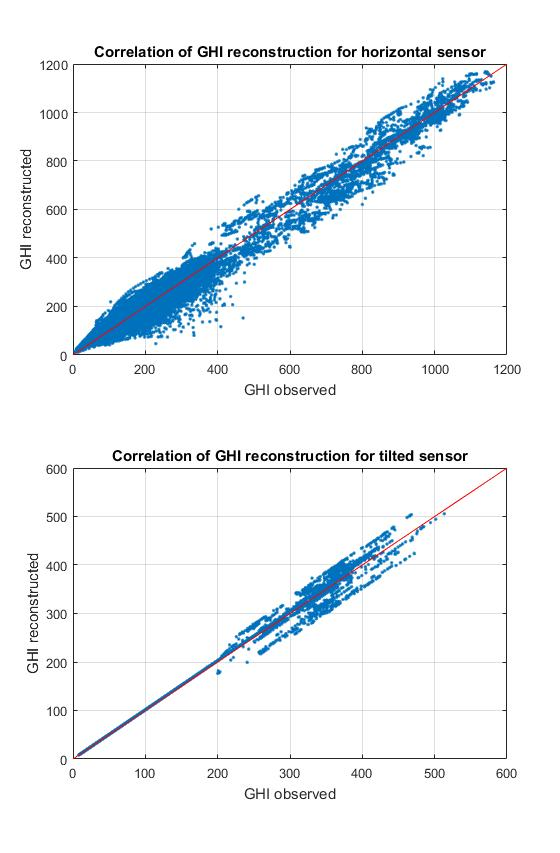
\includegraphics[scale=.5]{GHI_reconstructed}
\centering
\end{figure}

The hope was that by using the tuned version of Eq \ref{eq:GHI_reconstruct} and feeding it with GHI measurements of both irradiance sensors ( $GHI_1$ and  $GHI_2$) , we would be able to estimate DNI and DHI by multiplying GHI to inverse of coefficient matrix. In other word, we would be able to determine DHI and DNI for any situation including sun-flag=2 and sun-flag=3 which we excluded earlier for convenience. However, the results of this experiment was not satisfactory to hold our hypothesize. This could partially be due to the fact we are using DHI of tilted sensor instead of DNI of sensor 1 in this equation. Anyways,   the result of DHI and DNI for sun-flag=1 and 4 is still valid and we should now try to estimate these values from images.

The idea is that as we limit the effect of clouds on DNI by assuming $DNI=0$ or $DNI=DNI_{clear\_sky}$ in occlusion or not occlusion situations, the only way that clouds can affect GHI is through DHI variations. In next section we investigate characteristic of clouds in images to understand this effect better.

\section{Key factors influencing DHI}
\label{sec:img-features}
As we have shown in Figure \ref{fig:clean_sky_day_irr} all the irradiance components including DHI follow a bell-shape curve during a clear day and this curve varies throughout a year -lower in winter, higher in summer. We call these factors, \textbf{non-image} features as they are not obtained from images and are independent of cloud characteristics. We formulate these features as following:
\begin{itemize}
%\item Day of the year; defined as the number of days between query time and the first day of August.
%\item Time of the day; defined as the number of minutes passed the midnight at query time
\item $DHI_{clear sky}$
\item Zenith angle of the sun; between around 20 up to around 80 degrees
\end{itemize}
Even though $DHI_{clear sky}$ is dependent on zenith angle, but experiments show including both in the features list is beneficial.
\newline

Besides non-image features, we extract some visual features from sky images to help estimating DHI in not-clear situations. For image-based features there are several intuitions about what factors might affect DHI most. These includes cloud coverage, cloud type, shininess of sun, cloud color and etc. However, using cloud color features is not a good idea for our application, since they vary a lot even in very short-time ahead and predicting cloud color is not accurate enough. And since the aim of this study is to forecast irradiance for predicted cloud states in several minutes ahead, we restrict our image-based features to highly predictable features. This includes:
\begin{itemize}
\item sun-flag; as we explained in section \ref{sec:sun-states}, it is an integer number between 1 and 4. However, we only consider states 1 and 4. 
%\item Total cloud coverage; defined as the percentage of image pixels which are classified as cloud (i.e. 100\% for full cloud coverage, 0 for no cloud)
\item Semi-local cloud coverage; defined as the percentages of cloud pixels (i.e. image pixels which are classified as cloud) in four parts of the image separately, i.e. top right, top left, bottom right, bottom left. For each region, 100\% indicates full cloud coverage and 0 means no cloud. More information is given in section \ref{sec:cc_around_sun}.
\item Cloud coverage around the sun; defined as the percentage of image pixels in a small circle around the sun which are classified as cloud. This feature is explained in more detail in section \ref{sec:cc_around_sun}.
\item Saturation factor; defined as the percentage of saturated cloud pixels (i.e. with very high brightness). For complete description of this feature refer to section \ref{sec:saturation}.
\end{itemize}

\subsection{Cloud coverage features}
\label{sec:cc_around_sun}
For designing a cloud feature we took several issues into consideration. Firstly, this feature should be not too sensitive to the position of clouds, since clouds are very dynamic and position sensitivity will lead to not consistent feature vectors for actually similar cases in terms of DHI. Secondly, the relative position of clouds should be taken into account in the feature, for example clouds which are close to sun are most probable to reflect the irradiation than clouds in other parts. As a middle-ground for this two conditions we initially designed a feature vector that is sensitive to clouds position but not too much. For that, the image is divided into four equal part by connecting the central point to middle of each side. Then, a feature vector with four elements is created consisting of cloud coverage percentage for each part. However, this feature does not put enough emphasis on cloud variations around the sun which is desired for reflection situations. Therefore, another feature is created for cloud coverage in a circle around the sun. Since this circle is small (40 pixels radius), position of clouds is not likely to cause considerable difference on DHI, thus we calculate the cloud percentage in this circle around the sun as a one value feature between 0 to 100. Note that pixels that are classified as neither cloud nor sky, are most probably sun. Therefore, these pixels are not included in total number of pixels when calculating the cloud coverage percentage. The intuition is that cloud coverage around the sun is more important that total cloud coverage for DHI, since those clouds usually reflect more sunlight to the ground. The areas for extracting cloud coverage features are illustrated in Figure \ref{fig:cloud_coverage_features}.

\begin{figure}[h]
\caption{Regions of interest for extracting cloud coverage features}
\label{fig:cloud_coverage_features}
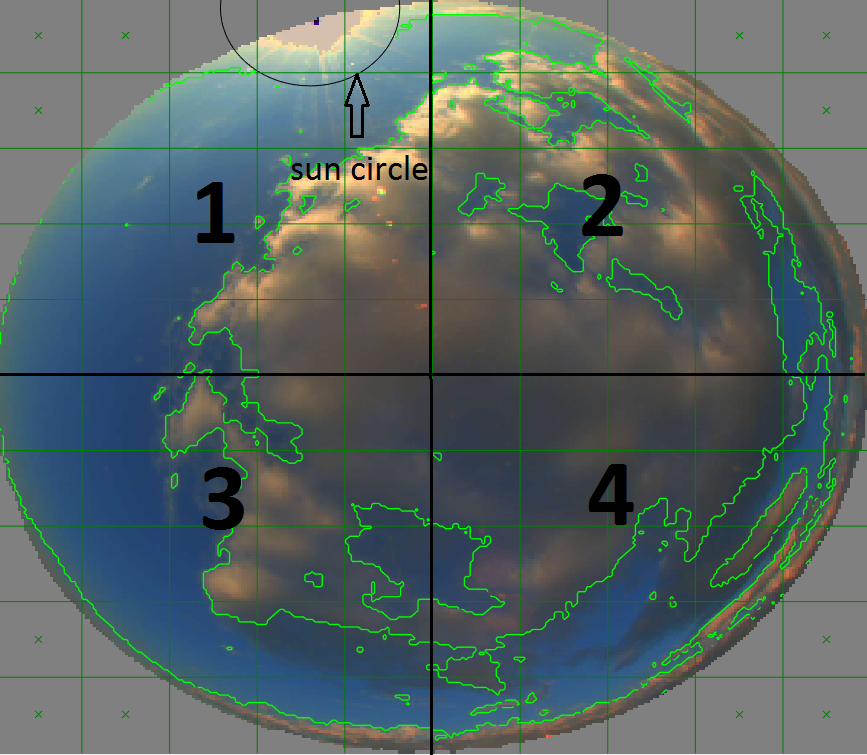
\includegraphics[scale=.5]{cloud_coverage_features}
\centering
\end{figure}

\subsection{Saturation factor}
\label{sec:saturation}
In some images that sun is occluded by a relatively thin cloud, we can see some pixels around position of sun, which are in fact part of the cloud but are very much illuminated by the sunlight which is passing through them. One example of this effect is shown in Figure \ref{fig:saturated_example}. 

\begin{figure}[h]
\caption{One example of saturated cloud pixels}
\label{fig:saturated_example}
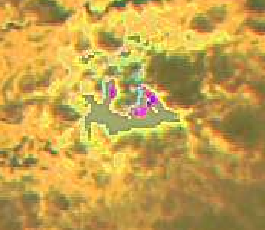
\includegraphics[scale=.5]{saturated}
\centering
\end{figure}

Even though, the sun is not directly visible int these images, resulting in DNI=0, our DHI observations show a considerable improvement in such cases. Therefore, we hypothesize than measuring this saturated pixels can be valuable feature vector for DHI estimation. Depending on the cloud type, and sun position these saturated areas can be predicated in very close future. That makes such feature valid for our forecast application. For calculating this feature we visually inspected many samples and realized that in all of them there is a very hight brightness band around the saturated regions which is even brighter than the saturated pixels. Based on this observation we designed the following algorithm for measuring saturation factor in any image. Firs, we crop an 120X120 pixel area around the sun as the only place saturation can occur. We convert this RGB patch into gray-scale and then find the pixels with intensity values more than 215. This threshold is been set empirically. These pixels are representing a contour for the saturated area. Since there are some discontinuity is this contour, we do the following approximation to find area inside. Every pixel in the patch is considered inside the contour, if that pixel or one of its side-neighbors (i.e. right or left) is bounded by at least 3 contour pixels in different directions (top,down,left,right). The results show that approximates saturated area is very close to actual area in the images. Finally, the saturation factor feature is calculated as the percentage of saturated pixels with respect to total patch pixels. This percentage is bounded to 60\% to comply with visual observation and reduce effect of errors in the detection algorithm. One example of detected saturated area is depicted in Figure \ref{fig:saturated_result_example}.

\begin{figure}[h]
\caption{Detected saturated area in a patch around sun}
\label{fig:saturated_result_example}
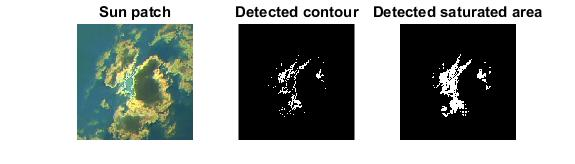
\includegraphics[scale=.5]{saturation_detect}
\centering
\end{figure}

Our final feature vector for each sky image consists of all the non-image and image-based features, resulting in a 9-element vector. Due to time limitation, we did not investigate cloud type or cloud texture pattern features.

\section{Dataset}
As it was mentioned in section \ref{sec:data}, we have data records and images from August 2015 until present for every 8 seconds during the day. Since we created our feature vector dataset in February 2016, the time span of images are from August 2015 to February 2016.  As we showed in Figure \ref{fig:calc_DHI_day}, HDI calculated values in the morning and evening are not accurate, therefore we skip these times in our final dataset. Furthermore, since estimating DNI for images with sun-flag 2 and 3 is too difficult and there is not ground-truth information for verifying results, we decided to restrict our data to only images with sun-flag 1 and 4, which corresponds to sun not visible and complete shining sun visible, respectively. This restriction reduces our usable data sample around 30\%. We also prune our data set to remove data samples that are too close to each other both in time and cloud conditions. For that, we iterate through images of each day for sampling a data set, but change the sampling rate by amount of change in cloud coverage from last sampled image to current one. This means that if there is long steady sunny condition during a day, we only sample handful of them. The same goes for continues full cloud coverage times during a day. On the other hand, when the cloud condition is changing a lot, we take more data samples to diversity our dataset and include as many variation of cloud situation as we can. The final data set after all these pruning, includes around 44,000 data samples from many different cloud conditions and many days from summer to winter.

\section{Learning the relation between image features and DHI}
In previous sections we approximated DHI from the pyranometers and also created a feature vector representing an image. Now, we need to find a way to relate them to each other in order to be able estimate DHI values from a given feature vector. Since DHI values are real numbers, this is a regression problem. 
Therefore, for we used several regression methods for solving that to find the best performing regressor on this particular problem. Because the domain value of our feature elements is different, we normalize every feature to [0,1] range before feeding it in any regressor algorithm. 

\subsection{Linear Regression}
\label{sec:lin_reg}
We tried linear regression to determine if DHI can be written as a polynomial function of feature vectors lile in Eq \ref{eq:linear_regress}.

\begin{equation}
\label{eq:linear_regress}
y_i = \beta_{1}x_{i1} + \ldots + \beta_{p}x_{ip} + \epsilon_{i}
\end{equation}
Where $y_i$ is DHI and $x_i$ is a feature vector. Also, square ($x^{2}$) and square root ($\sqrt(x)$) of features are added to the feature list to evaluate non-linear relation of features to target as well. To consider mutual relation of features, interaction of features (i.e. $x_{i}x_{j}$) were added to final feature list, resulting in 63 element feature vector. To prevent cluttering the features any further, we did not evaluate logarithmic or exponential of features.

\subsection{K-nearest-neighbors (K-NN) Regression}
Another approach that we tried was K-NN regression. This method aims to find unknown target value of a feature vector by calculating a weighted average of target values from K training feature vectors that are most closest (i.e. neighbors) to the query feature vector in the feature space. In other word, K-NN assumes that if two feature vector are very similar to each other based on a similarity measure, then their target should be similar too. And this is a valid assumption for our application. These neighbors of input vector are weighted by the inverse of their distance for averaging. The distance between feature vectors can be defined arbitrarily, but popular distance choices for continues variables are Euclidean, Manhattan Eq. \ref{eq:manhattan_distance} and Minkowski Eq. \ref{eq:minkowski_distance}. We experimented all three of these distances to find the one with least error. Note that Minkowski distance is equal to Manhattan for $q=1$ and equal to Euclidean for $q=2$.
 To reduce the noise in data, usually the number of neighbors (K) for averaging should be 10 or more. However, the best K can vary depending on the data set. Therefore, we have tried several values to tune this parameter.

\begin{equation}
\label{eq:manhattan_distance}
d = \sum_{i=1}^{k} |x_i - y_i|
\end{equation}

\begin{equation}
\label{eq:minkowski_distance}
d = (\sum_{i=1}^{k} (|x_i - y_i|)^{q})^{1/q}
\end{equation}

\subsection{Support Vector Machine Regression (SVR)}
Even though Support Vector Machine\cite{svm_r} is best known for classification problem, but one can use a modified version of that for regression too with almost all the benefits of normal SVM. In SVR formulation two maximum margin hyperplanes are found between negative and positive errors between a polynomial function of input features and the target values. In the soft-margin SVM which we are using, the $\epsilon$ parameter helps to tolerate small errors and find better support vectors. Slack variables help to ensure existence of a convex solution as well as reducing the effect of noise in data. Kernels in SVR map the feature space to a higher dimensional space that might be more suitable for finding those separating hyperplanes. Since we are working with images and there is a lot of noise in features as well, a Radial Basis Function (RBF) kernel is used which can help smoothing these noise and find better hyperplanes. The gamma parameter ($\gamma$) in RBF kernel defines how far the influence of a single training example reaches, with low values meaning far and high values meaning close. The gamma parameters can be seen as the inverse of the radius of influence of samples selected by the model as support vectors.


\subsection{Training and test datasets}
For every learning algorithm we need to have a separate training and testing dataset. Since usually Linear Regression and K-NN need large training set size to avoid over-fitting and also smooth the noise in data, we dedicate 40\% of our data samples for training set, and the rest for testing. This means the training dataset has around 18,000 data samples and test dataset has around 26,000 data samples. For the case of Support Vector Machine Regression, there is no need for such a big training size due to $\epsilon$ and slack variables as well as kernel non-linear mapping. However, for the sake of comparability of results, we use the same training and test sets for all three methods. The distribution of DHI (target) values in our dataset is not uniform. There are many more samples at low values of DHI than high values. Therefore, to make sure that there is enough sample from every DHI range in the training and test sets, we partition the DHI values into 5 ranges, [0,100], [100,200], [200,300], [300,400], [400,500]. Then in any range we choose $N/5$ of samples randomly for training where $N$ is total number of training. If the number of samples in a range is less than $N/5$ we take 70\% of the sample in that range as training and the rest as test. Using this sampling trick, we provide enough samples from every DHI range in order to be able to estimate values in that range later with regression. In next chapter, we show some results of this three regression method on test set after being trained with training data.


%\section{Translating irradiance to power}
%\subsection{Estimating shadow ratio on the plant site}
%refer to Figure \ref{fig:overall_system_design_power}.
%Projecting plant coordinates into the sky using assumed cloud height
%Adaptation to smooth changes of power by using the histogram of irradiance over past 30 minutes
%\begin{figure}[h]
%\caption{Overall simple system design for power prediction}
%\label{fig:overall_system_design_power}
%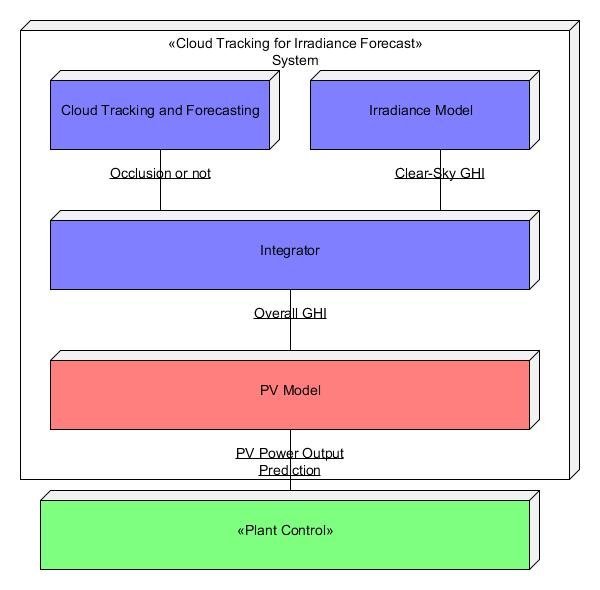
\includegraphics[scale=.5]{Overall_Simple_System_Design}
%\centering
%\end{figure}
